\documentclass{book}

\usepackage{amsmath}
\usepackage{amssymb}
\usepackage{amsxtra}
\usepackage{graphicx}
\usepackage{listings}

\newcommand{\refchapter}[1]{Chapter~\ref{#1}}
\newcommand{\refsec}[1]{Section~\ref{#1}}
\newcommand{\refeqn}[1]{Equation~(\ref{#1})}
\newcommand{\reffig}[1]{Figure~\ref{#1}}

\title{\bf C++ UI design for NAG Optimization Modelling Suite \\
{\small Group 6}} 

\author{Konstantin Korkin, Maksim Feldman, Tran Man Khang, \\Yifei Huang, Ziya Valiyev\footnote{Informatik 12: Software and Tools for Computational Engineering, RWTH Aachen University, {\tt info@stce.rwth-aachen.de}}}
\date{
\includegraphics[width=.6\textwidth]{rwth_i12_softw-werkz_en_rgb}}

\begin{document}

\lstloadlanguages{[ISO]C++}
\lstset{basicstyle=\small, numbers=left, numberstyle=\footnotesize,
  stepnumber=1, numbersep=5pt, breaklines=true, escapeinside={/*@}{@*/}}

\pagestyle{headings}

\maketitle

\tableofcontents

\chapter*{Preface}

\begin{itemize}
\item administrative information about the project (e.g, topic issued by which institute)
\item fit of topic into study program (e.g, sufficient prior knowledge)
\item acknowledgement of supervision
\end{itemize}

\chapter{Analysis} \label{ch:analysis}

\section{User Requirements}
This C++ interface ought to be made to to define and solve optimization problems with the help of the NAG Optimization Modelling Suite (NOMS).\\
The users would like to expect the software to firstly define the objective function and the constraints they give to the interface and then solve the optimization problem by itself without having the users to put in any code or derivatives of the function. Namely the software should be able to choose the appropriate solver for a specific optimization problem.\vspace{1em}\\
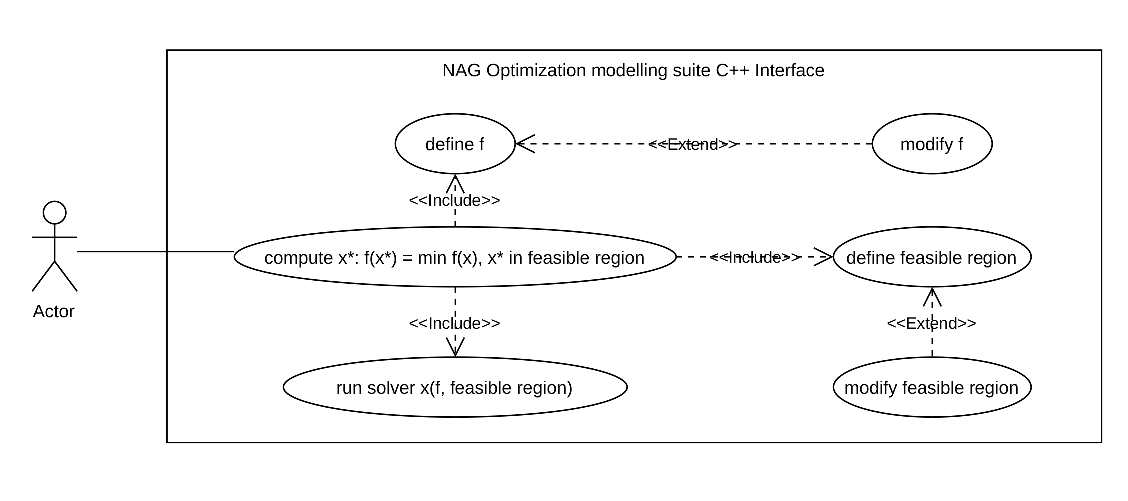
\includegraphics[width=\textwidth]{use case.pdf}
\vspace{1em}\\
The use case diagram above shows how the interface is supposed to process such a task of solving an optimization problem. To find an extreme of the function $f$, it defines the function and the feasible region which could be modified, then it chooses a certain solver to compute the extreme $x^{*}$. The user don't have to identify what kind the problem is (linear, non-linear) nor choose the right solver themselves to solve it. 


\section{Essential Technical Background}

includes references into literature, e.g, \cite{Ries1522Rad}

\section{System Requirements}
Functional:
\begin{itemize}
\item defining optimization problems, including:
	\begin{itemize}
	\item the ability to define and modify objective functions
	\end{itemize}
\item automatic computation of derivatives
\item recognisation of linear contraints
	\begin{itemize}
	\item automatic modification of problem to reflect linearity
	\end{itemize}
\item solve problems with either automatic solver choice or manual choice from the 3 solvers: e04mt, e04kf, e04st
\end{itemize}
Nonfunctional:
\begin{itemize}
\item backend: NAG Optimization Modelling Suite, C++ interface
\item interface implementation in C++ using OOP
\item testing with CTest and googletest
\item documentation with doxygen
\item automatic computation of derivatives and recognisation of linear contraints with dco/c++
\end{itemize}

\chapter{Design} \label{ch:design}

\section{Class Candidates}
includes libraries that you built on explained briefly and references to further information\\
Some keywords/classes from the existing C++ interface in the NAG optimization modelling suite (NOMS)\footnote{\tt https://www.nag.com/numeric/nl/nagdoc\_latest/flhtml/e04/e04intro.html\#optsuite} which could be used as classes in ours:
\begin{itemize}
	\item problem
	\item solver
	\item dco/derivative
	\item bound
	\item function
		\begin{itemize}
			\item objectiveFunction
			\item constraintFunction
		\end{itemize}
	\item linearInfo
\end{itemize}

\section{Class Model}
UML Class diagram(s) and description; should link into overall design through
reference of application programming interfaces (API) of third-party software\\
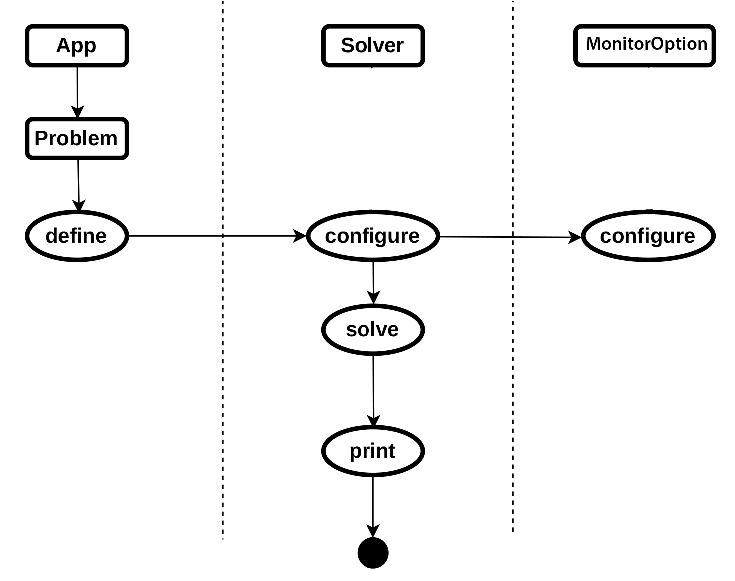
\includegraphics[width=0.9\textwidth]{Class Model - Optimize function.pdf}\\
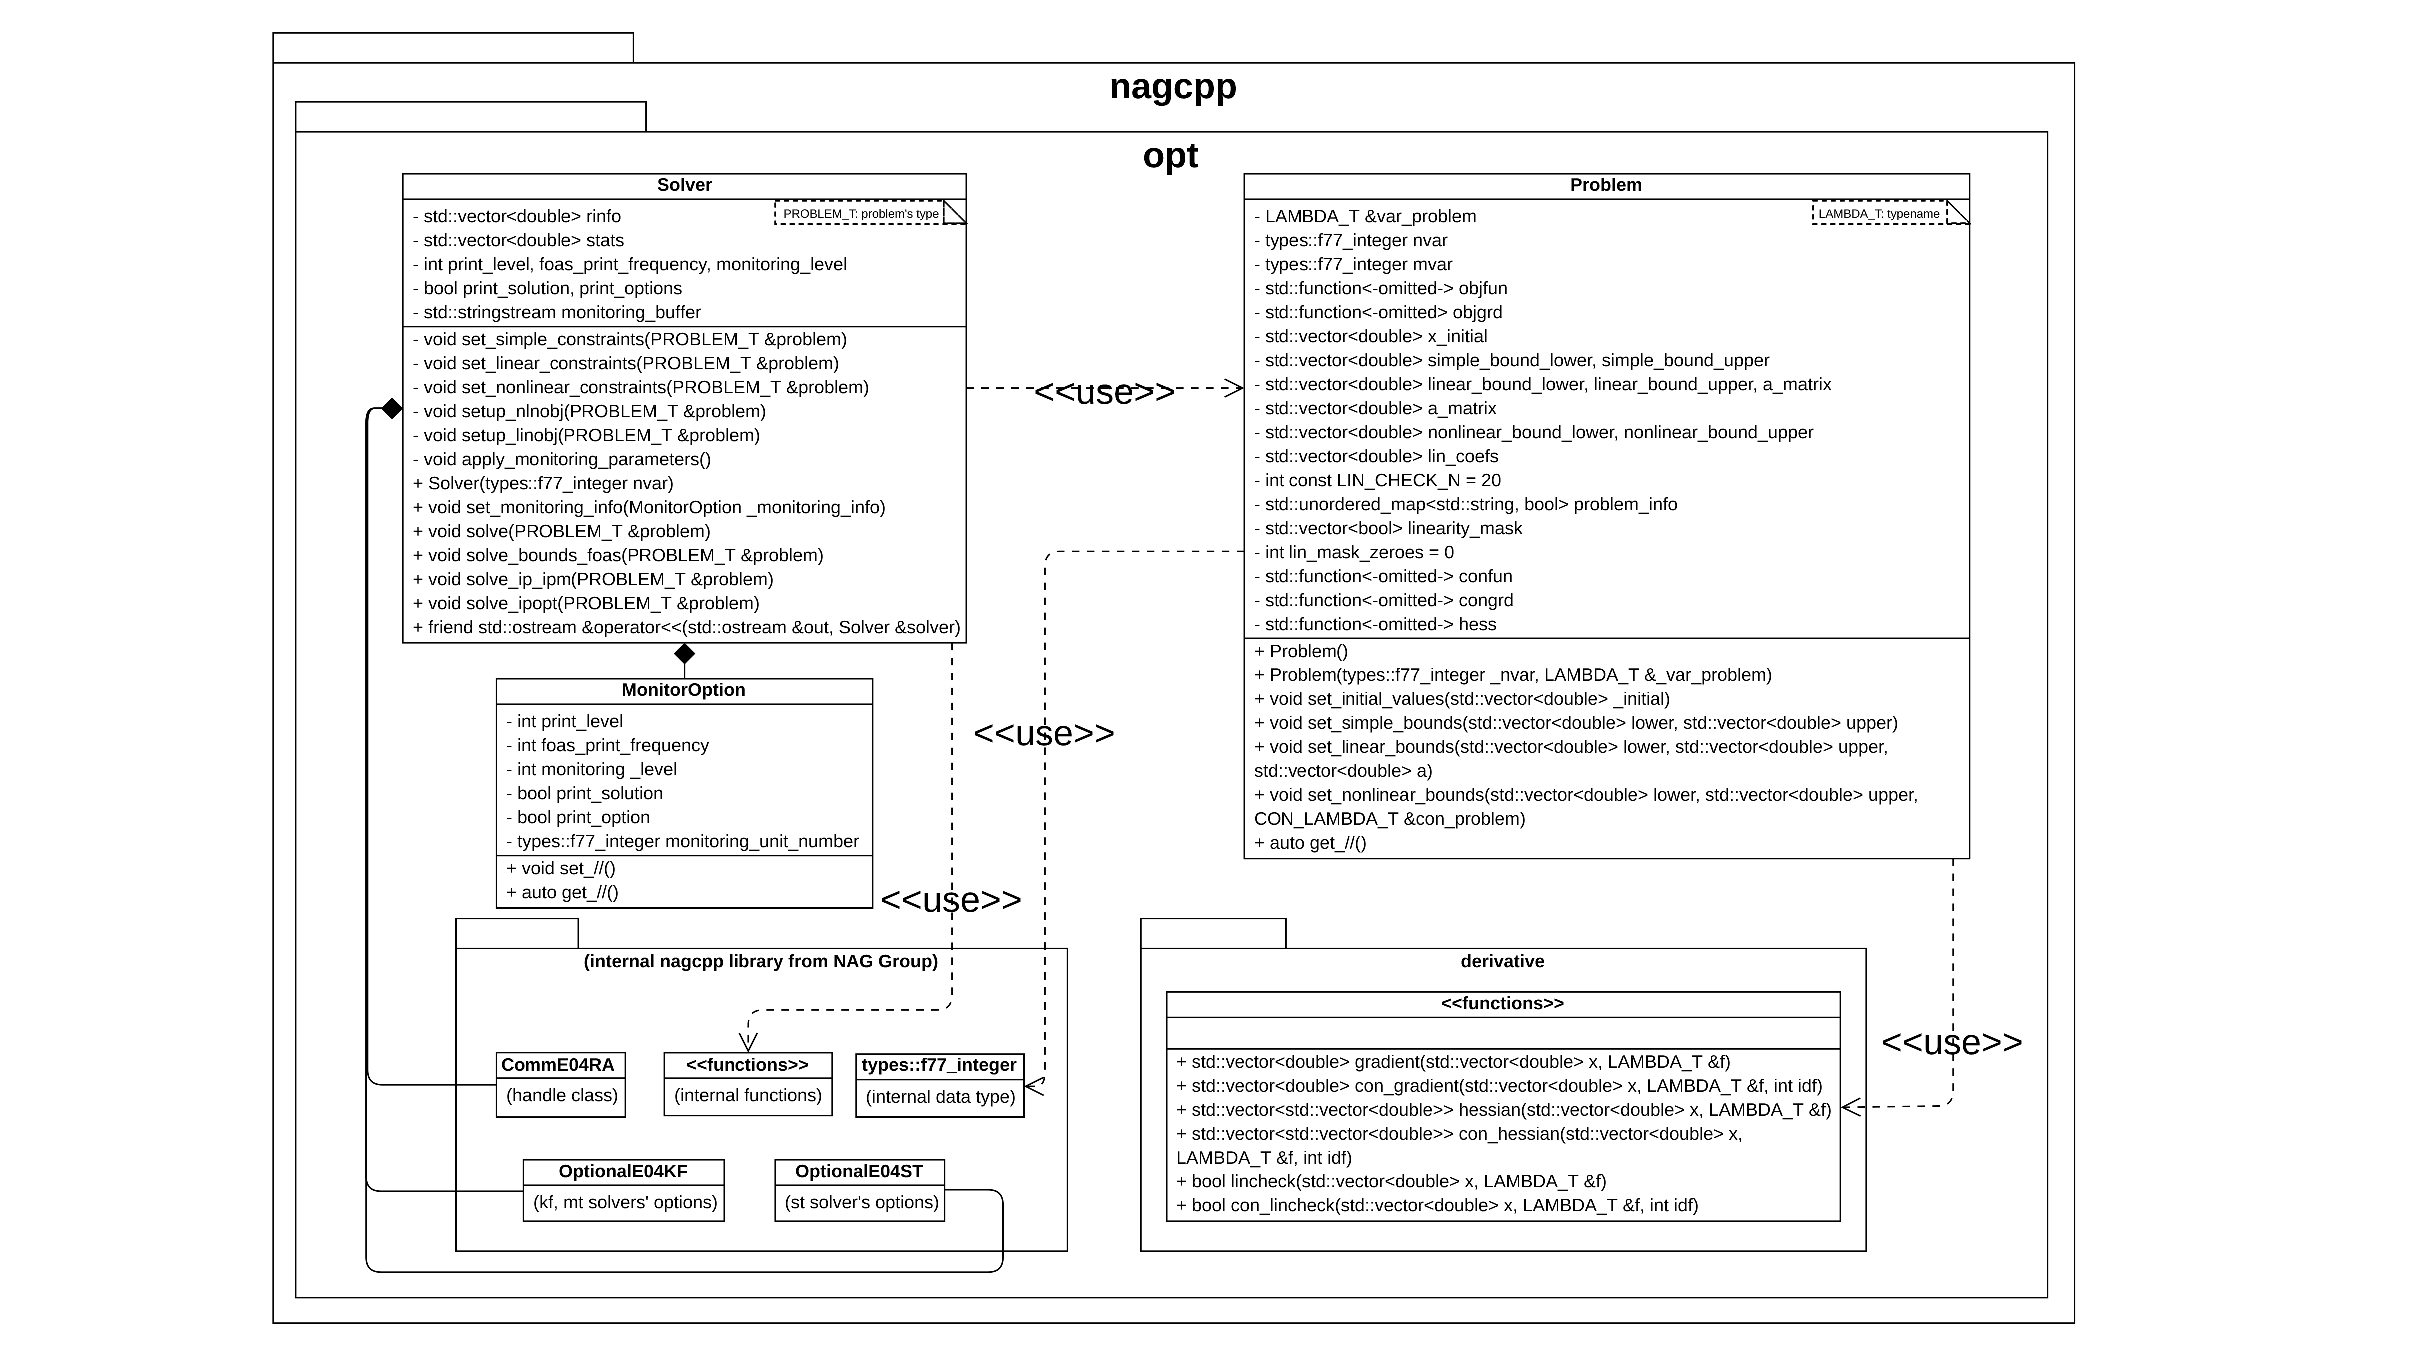
\includegraphics[width=\textwidth]{class diagram.pdf}\\

\chapter{Implementation} \label{ch:implementation}

\section{Development Infrastructure}
\begin{itemize}
	\item Target platform: Linux devices, specifically the Virtual Machine provided by Prof. Naumann
	\item Programming language: C++ 20
	\item Compiler: gcc
	\item Build system: CMake
	\item Runtime library: NAG Library with C++ interface, dco/c++, the standard ones (std, math.h, etc.)
\end{itemize}

\section{Source Code}

overview of source code structure (file names, directories); build instructions; references into source code documentation e.g, doxygen\footnote{\tt https://github.com/doxygen/doxygen}; short (!) code listings 
\begin{lstlisting}
#include<iostream>
int main() {
  std::cout << "Leave me alone world!" << std::endl;
  return 42;
}
\end{lstlisting}
only if helpful (must come with detailed explanation)

\section{Software Tests}

e.g, googletest\footnote{\tt https://github.com/google/googletest}

\chapter{Project Management} \label{ch:projectmanagement}
\begin{figure}
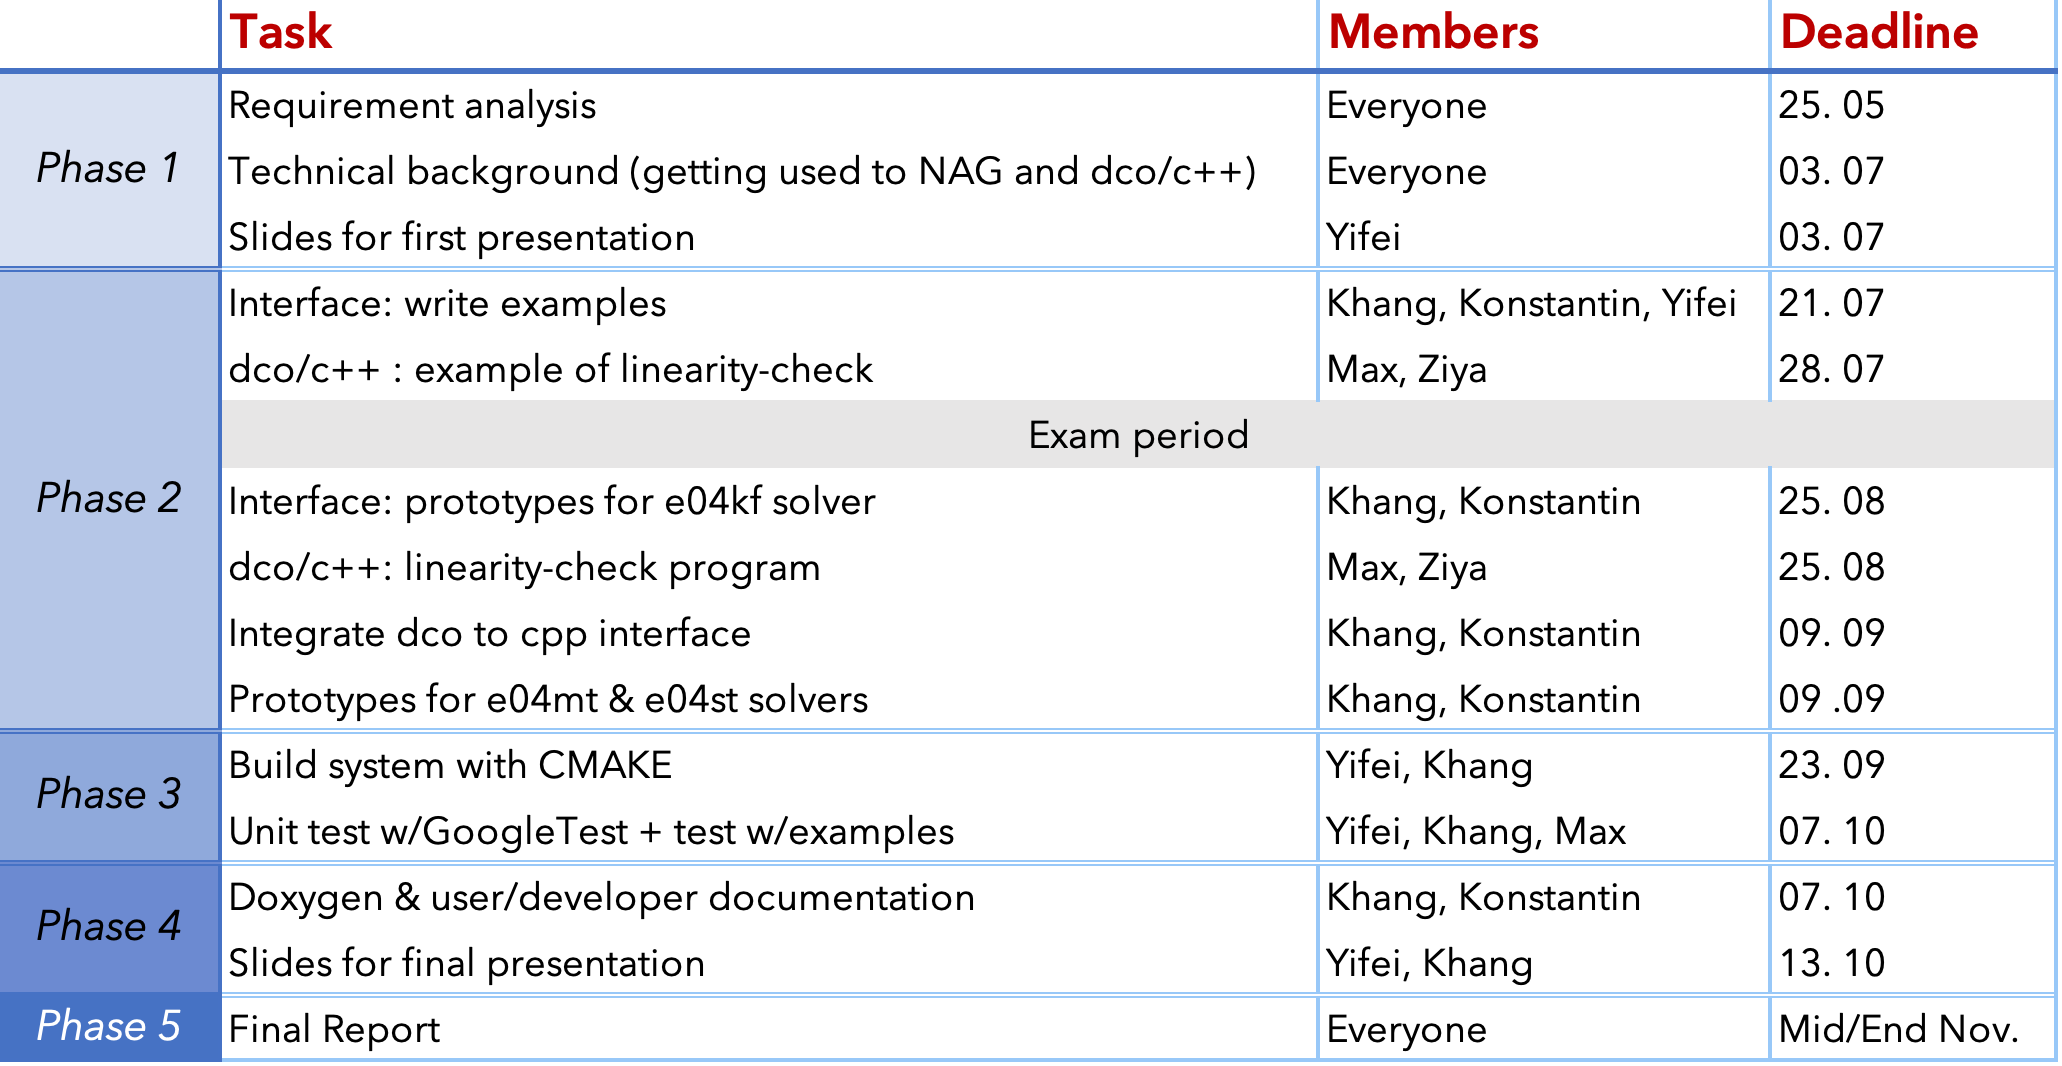
\includegraphics[width=\textwidth]{proj_management.png}
\caption{\small Project Management table}
\end{figure}\par
\hspace{4ex}Our project workflow was devided into five phases in a time span of 6 months: analysis, design and implementation, testing, documentation and final report writing. \par
\vspace{1em}
At the start of this project, we discussed and worked together for the requirement analysis and technical background so that everyone could have the basic understanding of the project assignment and also get to know the NAG library for later development. At the beginning of July, we then presented the requirement analysis of our project and came up with  preliminary division of work of the rest phases. \par
In the design and implementation phase, Khang and Konstantin took charge of the main C++ interface (prototypes for the three solvers, etc.) and implemented the code in C++20 whilst Ziya was responsible for applying dco/c++ for automatic differentiation and linearity check. Despite the one-month-long exam period for all members, we still managed to stick to our plan. \par
After the source code was implemented and runned successfully with all the expecting features, Yifei constructed a build system based on CMake\footnote{\tt https://cmake.org/} and Khang optimized the system to make it aesthetically well-structured. Meanwhile, Yifei and Khang looked into googletest\footnote{\tt http://google.github.io/googletest/} and CTest to create unit-tests for the interface, together with Valgrind to ensure it was free of memory leaks and invalid memory accesses. Max implemented three examples for each solver to assure us of the functionality of the interface. \par
Before the final presentation of the project, Khang and Konstantin worked on user- and developer-documentation with doxygen\footnote{\tt https://github.com/doxygen/doxygen} as they were the most familiar with the source code. With Khang summarizing and arranging the content of the presentation, Yifei made the slides in \LaTeX\ for both presentation and also the report of the project. \par
\vspace{1em}
As a group, we kept our communication both internal and with our supervisor Johannes, managed the time and overcame exceptional situations such as sickness, which was precious experience in software development for all of us.\par
We sticked to our roles as originally planned and made sure to have both online group meetings every week to discuss and online meetings with our supervisor every 2 week to have them check on our progress so that everything was kept on track very well. To keep everything up-to-date on everyone's end, we made good use of git\footnote{\tt https://git.rwth-aachen.de/tranmankhang1705/nag-optimization-modelling-suite-ui} for software version control. As a prevention of unexpected circumstances, tasks were always assigned to a pair of our group members. If one person is unavailable, there is still another to keep up, which proved much of use.


\bibliographystyle{plain}
\bibliography{literature}

\appendix

\chapter{User Documentation} \label{ch:userdoc}

\section{Building}

e.g, using cmake\footnote{\tt https://cmake.org/} and make\footnote{\tt https://www.gnu.org/software/make/}

\section{Testing}

e.g, \verb!make test!

\section{Running}

documented sample session(s); e.g, \verb!make run!

\end{document}

